\documentclass[11px, a4paper]{article}
\pagestyle{empty}
\usepackage{amsmath, amssymb}
\usepackage{float}
\usepackage{graphicx}
\usepackage{enumerate}
\usepackage{hyperref}
\usepackage[left = 0.2in, right = 0.2in, top = 1in, bottom = 1in]{geometry}
\parindent 0px

\title{PRACTICE \LaTeX}
\author{Joel Mwala}
\date{\today}


\begin{document}
\maketitle
\tableofcontents
\section{Day One}
\subsection{formulaes}
$$E = mc^{2}$$
$$2x^{34}$$
$$2x^{2x+4}$$

\subsection{Greek letters}
$$\pi$$
$$\Pi$$
$$\alpha$$
$$\omega$$
$${\pi}r^2$$

\subsection{Functions}

$$y = mx+c$$
$$y = {\sin}^2 (x)$$

$$\sqrt[4]{x+1}$$
$$\sqrt{16}$$
$$\sqrt[4]{1 + \sqrt{x}}$$

\subsection{Fractions}

$$\frac{2x+3}{\sqrt{5}}$$
$$\arctan x$$
$$\ln 15$$
$$\sqrt{(x_2-x_1)^2+(y_2-y_1)^2}$$\\[6pt]

the fraction is $\dfrac{3}{5}$ which means \\[6pt]
$${a, b, c}\in \mathbb{R}$$
$$\left |\frac{8}{1 + \frac{\sqrt{3}}{7}}\right|$$\\[19px]

\subsection{Tables}


\begin{tabular}{|c||c|c|c|c|}
    \hline
    $x$    & 1 & 2 & 3 & 4  \\ \hline
    $f(x)$ & 2 & 4 & 8 & 16 \\ \hline
\end{tabular}

\vspace{1cm}

\begin{table}[H]
    \centering
    \def\arraystretch{1.5}
    \begin{tabular}{|c||c|c|c|c|}
        \hline
        $x$    & 1             & 2 & 3 & 4  \\ \hline
        $f(x)$ & $\frac{1}{x}$ & 4 & 8 & 16 \\ \hline
    \end{tabular}
    \caption{values for $f(x) = x^x$}
\end{table}

\begin{align}
    5x + 6 & = 26     \\
    5x     & = 26 - 6 \\
    x      & = 4
\end{align}

\begin{align*}
    5x & = 20
\end{align*}
\section{Day Two}
\subsection{Lists}

\begin{enumerate}[A.]\setcounter{enumi}{3}
    \item Books
    \item Pencils
    \item Pens
    \item Soap
          \begin{enumerate}[1)]
              \item Books
              \item Pencils
              \item Pens
              \item Soap
                    \begin{enumerate}
                        \item Books
                        \item Pencils
                        \item Pens
                        \item Soap

                    \end{enumerate}
              \item capial
          \end{enumerate}
    \item frista
\end{enumerate}
\vspace{2cm}
\subsection{formatting}

This will produce \textit{italicized} text  \\
This will produce \textbf{bold face} text   \\
This will produce \textsc{small caps} text  \\
This will produce \texttt{some code} text   \\
Please visit my website \href{http://www.joelmwala.tech}{joelmwala.tech}fr
\section{Images}
\begin{figure}[H]
    \begin{center}
        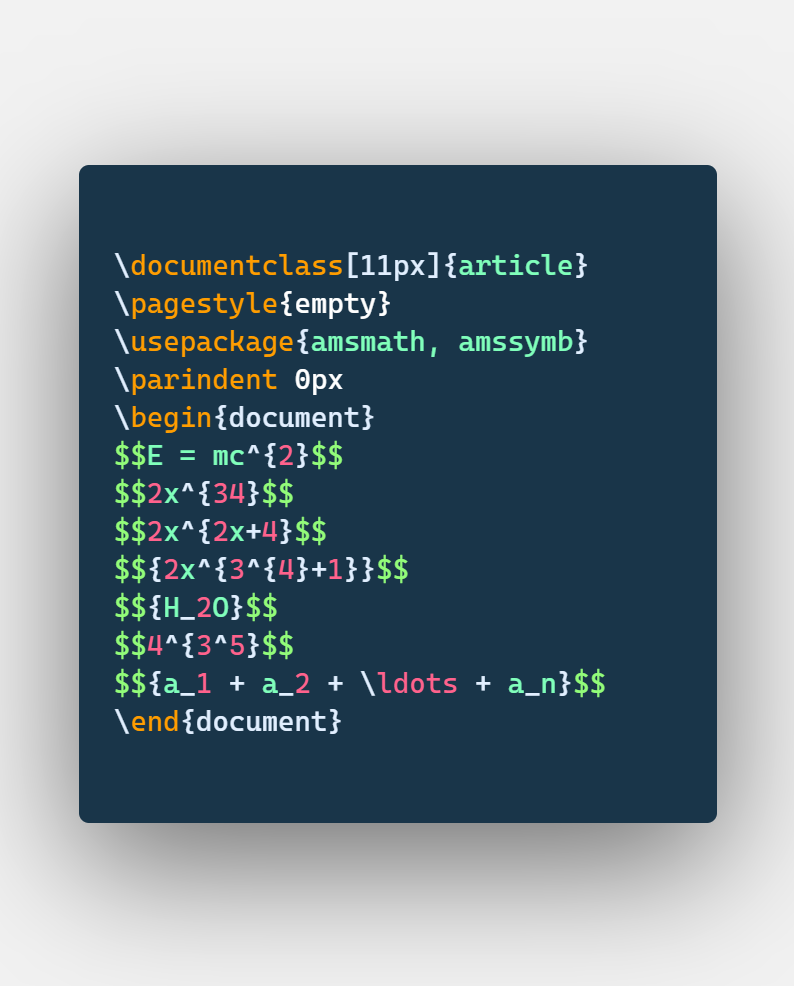
\includegraphics[width = 0.5\textwidth]{code1}
    \end{center}
\end{figure}


\end{document}